\section{TOF Matching Efficiency}\label{section:star_TOFeffi}
The TOF acceptance, hit reconstruction efficiency and matching efficiency with TPC tracks,  $\epsilon_\textrm{TOF}\left(p_\textrm{T},\eta,V_{z}\right)$, is defined as the probabilty that a~global TPC track, that pass the selection criteria and is associated to a~true-level primary particle, is matched with hit in TOF. The  single particle MC embedded into Zerobias data was used. The efficiency was measured as a function of $p_\textrm{T}$, $\eta$ and $V_z$, separately for each particle type, and is expressed as:
\begin{equation}
\epsilon_\textrm{TOF}\left(p_\textrm{T},\eta,V_{z}\right)=\frac{N_\textrm{reco}^\textrm{global-TOF}\left(p_\textrm{T},\eta, V_z\right)}{N_\textrm{reco}^\textrm{global}\left(p_\textrm{T},\eta, V_z\right)}
\end{equation}
where $p_\textrm{T}$, $\eta$, $V_z$ are quantities related to a~generated particle, $N_\textrm{reco}^\textrm{global}\left(p_\textrm{T},\eta, V_z\right)$ is the~number of reconstructed global tracks assigned to a given true-level primary particle, $N_\textrm{reco}^\textrm{global-TOF}$ $\left(p_\textrm{T},\eta, V_z\right)$ is the number of global tracks assigned to a given true-level primary particle and matched with a~hit in TOF.

\noindent The TOF efficiency for $\pi^-$ in three sample $V_z$ bins is shown in Fig.~\ref{fig:tofEffi}.
\begin{figure}[h!]
	\centering
	\begin{subfigure}{.49\textwidth}
		\includegraphics[width=\textwidth,page=3]{chapters/chrgSTAR/img/tofEff/Eff2D_TOF_pion_Minus.pdf}
	\end{subfigure}
	\begin{subfigure}{.49\textwidth}
		\includegraphics[width=\textwidth,page=11]{chapters/chrgSTAR/img/tofEff/Eff2D_TOF_pion_Minus.pdf}
	\end{subfigure}
	\begin{subfigure}{.49\textwidth}
		\includegraphics[width=\textwidth,page=18]{chapters/chrgSTAR/img/tofEff/Eff2D_TOF_pion_Minus.pdf}
	\end{subfigure}
	\begin{minipage}{.49\textwidth}
		\caption{TOF reconstruction and matching efficiency of $\pi^-$ in 3 sample bins of true $V_z$. Plots represent the TOF efficiency $\epsilon_{ TOF}$ as a function of $p_\textrm{T}$ and $\eta$ in single $V_z$ bin. Black lines and arrows indicate region accepted in analysis.}
		\label{fig:tofEffi}
	\end{minipage}
	
\end{figure}
%\FloatBarrier

\subsubsection{Data-Driven Correction to TOF Efficiency}
The TOF efficiency correction was obtained from the embedded MC. It was found that there are some inaccuracies in the description of real detector geometry in the STAR detector simulation. Therefore,  a~correction to the TOF efficiency was derived  by extracting  a~modified TOF efficiency  (using  tag\&probe method)  in the  same way from the \ac{CEP} of $\pi^+\pi^-$ data and embedded MC and comparing the results between each other~\cite{RafalThesis}. Figure~\ref{fig:tofEffiCorrection} shows the sample comparison of modified TOF efficiency as a function of $p_T$ between data and MC. The difference between these two was taken as an additive correction to the TOF efficiency estimated from embedded MC.

\begin{figure}[h!]
	\centering
	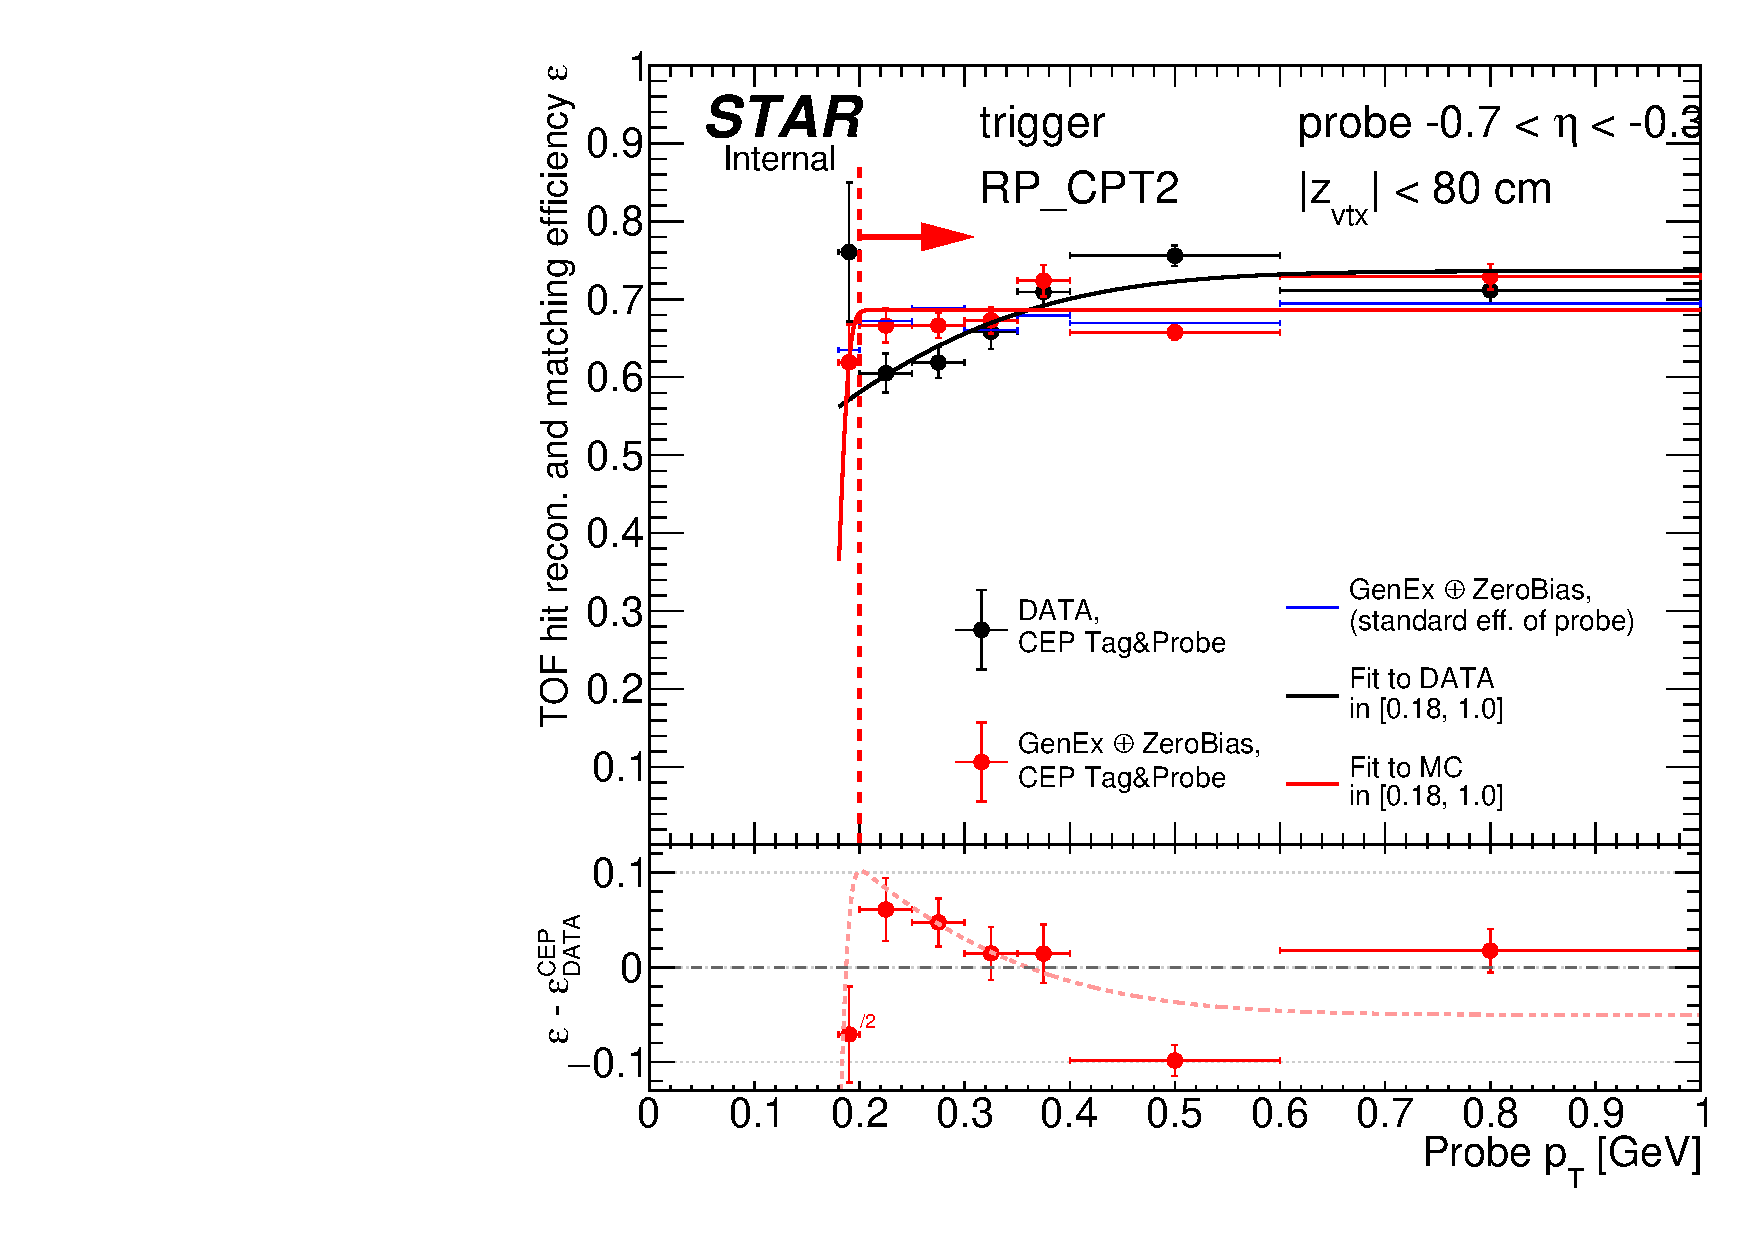
\includegraphics[width=0.49\textwidth,page=1]{chapters/chrgSTAR/img/tofEff/TofEffVsPt_eta_minus07_to_minus03_CPT2.pdf}
	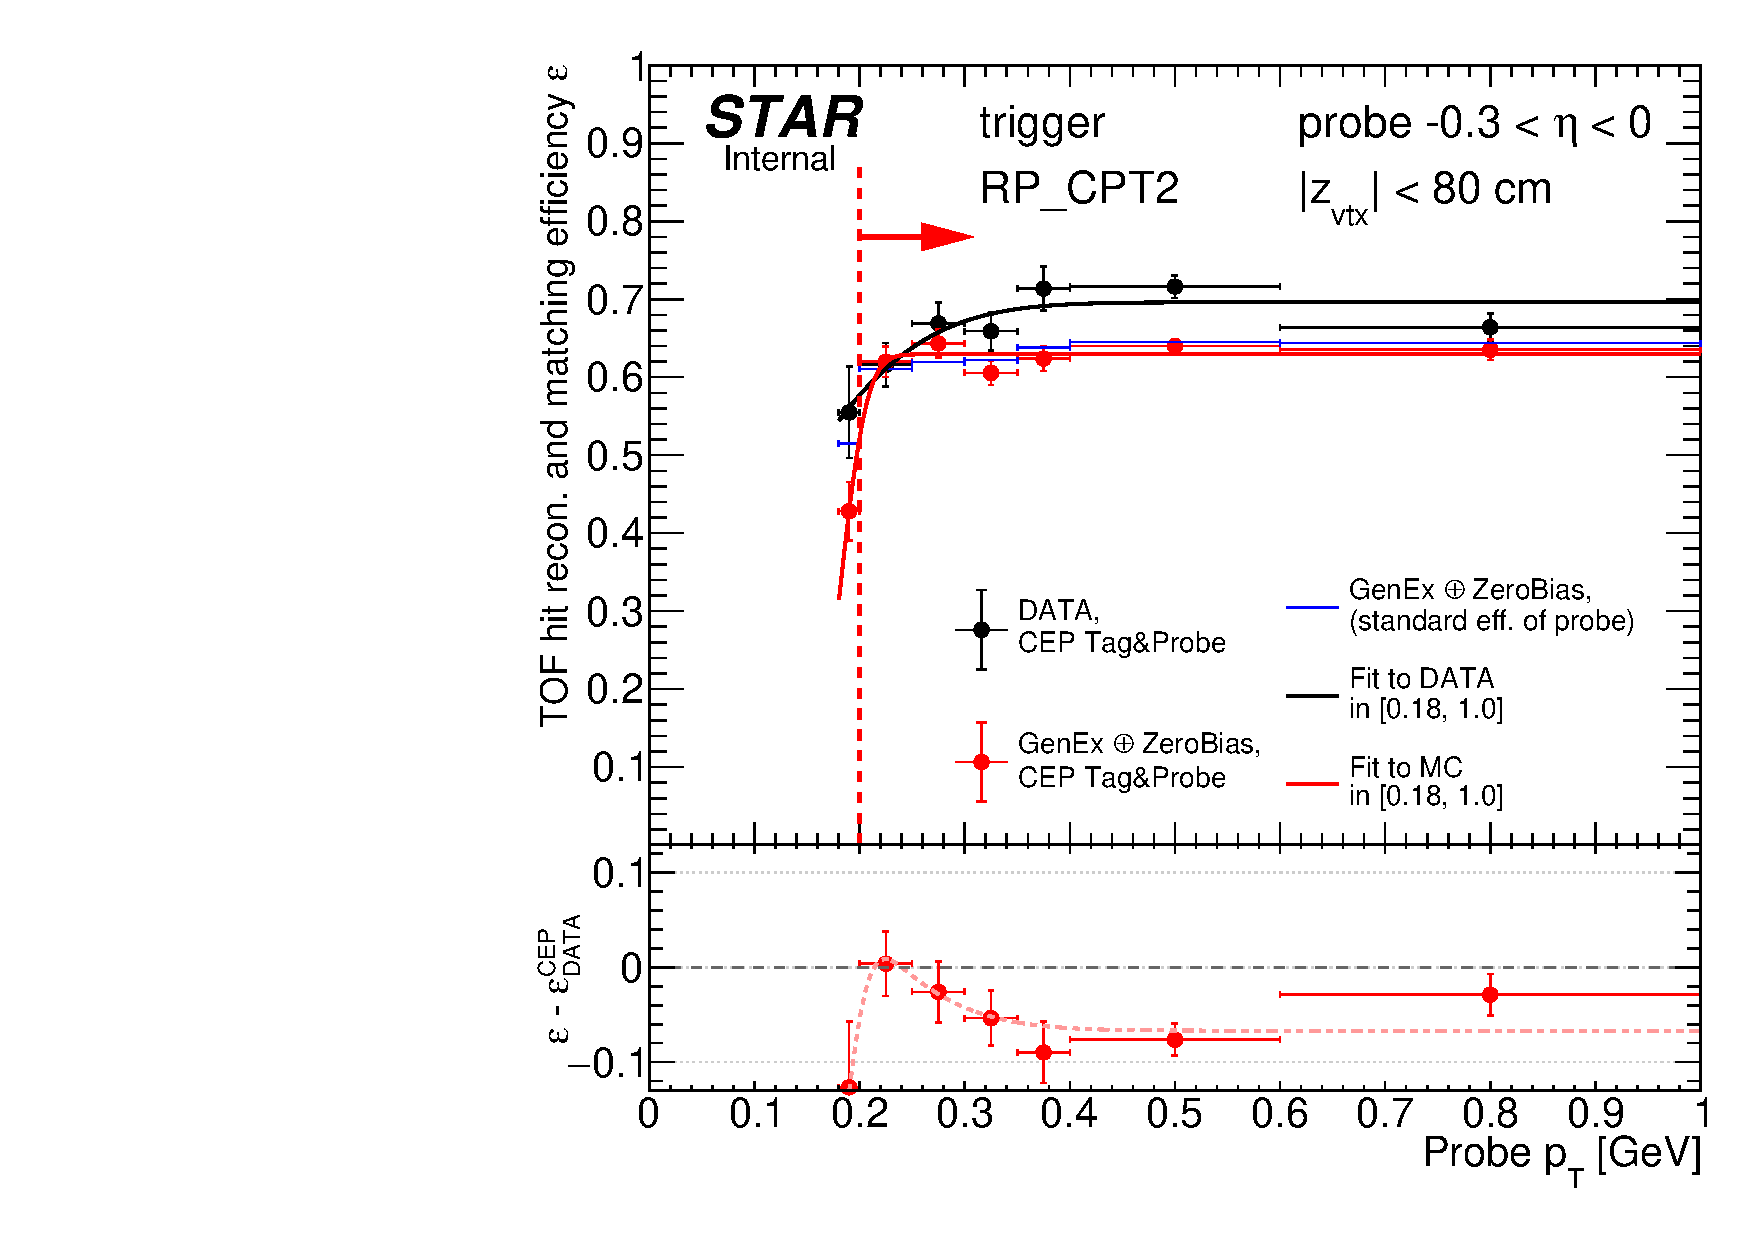
\includegraphics[width=0.49\textwidth,page=1]{chapters/chrgSTAR/img/tofEff/TofEffVsPt_eta_minus03_to_0_CPT2.pdf}
	\caption{Modified TOF efficiency from \ac{CEP} data compared with the result from embedded \ac{CEP} MC as a function of $p_\textrm{T}$. Blue lines denote the TOF efficiency calculated in the standard way. Differences between modified TOF efficiency from  embedded MC and data are shown in the bottom pads. Red lines with arrows indicate region accepted in analysis. Figure taken from~\cite{RafalThesis}.}
	\label{fig:tofEffiCorrection}
	
\end{figure}
%\FloatBarrier

%\subsubsection{TOF System Simulation Accuracy}
The systematic uncertainty on TOF system simulation accuracy was estimated by comparing the nominal TOF efficiency, including efficiency from single particle MC and data-driven correction, with the one obtained with an independent method. 

The alternative method uses TPC tracks cointaining hits in the HFT~\cite{RafalThesis}. Since the time of response of HFT is much shorter than of TPC, it is very probable that TPC tracks containing hits in HFT are real, in-time tracks. As a result, the alternative correction to  TOF efficiency correction was obtained. The difference between this correction  and the correction described in the previous paragraph was used as  the systematic uncertainty of the overall TOF efficiency, which is shown in Fig.~\ref{fig:tofEffiSyst}.
\begin{figure}[h!]
	\centering
	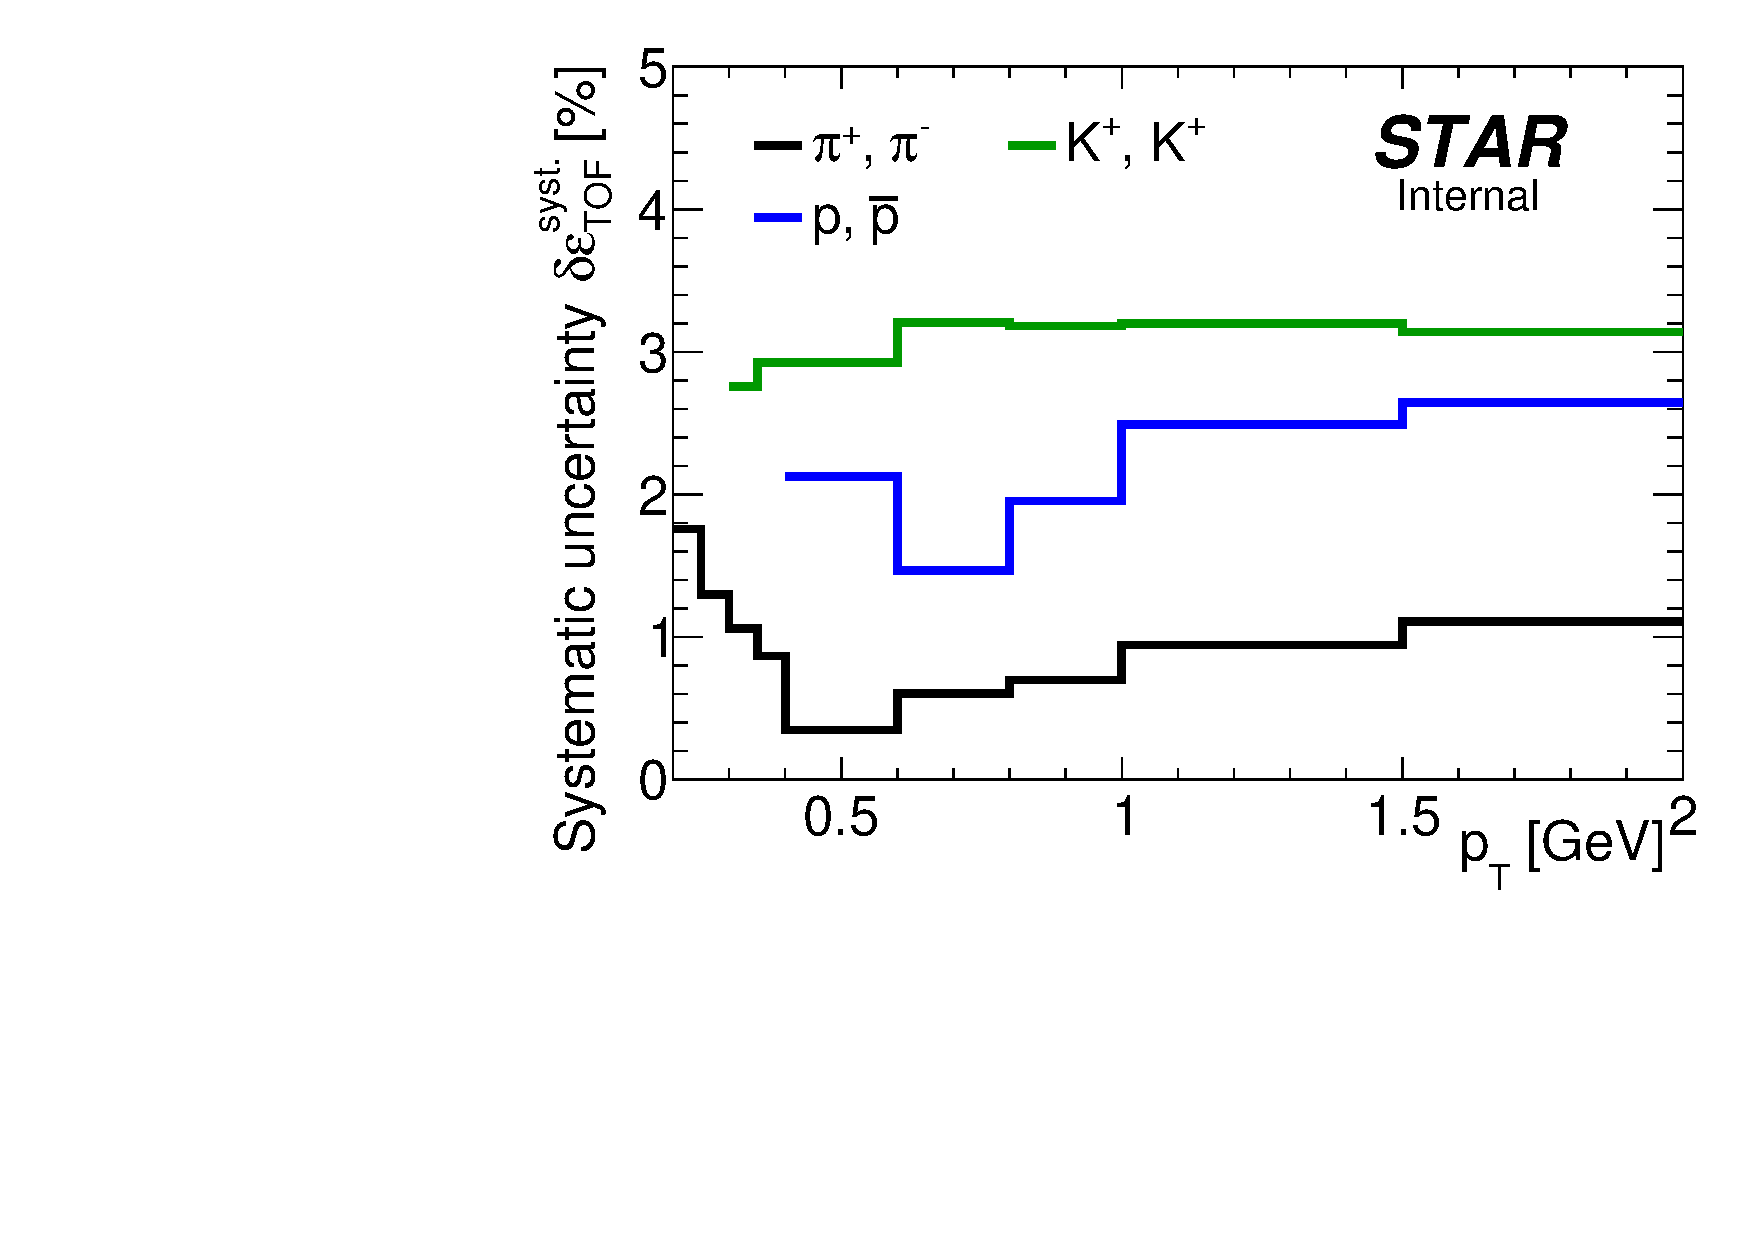
\includegraphics[width=0.49\textwidth,page=1]{chapters/chrgSTAR/img/tofEff/TofSystError_pT.pdf}
	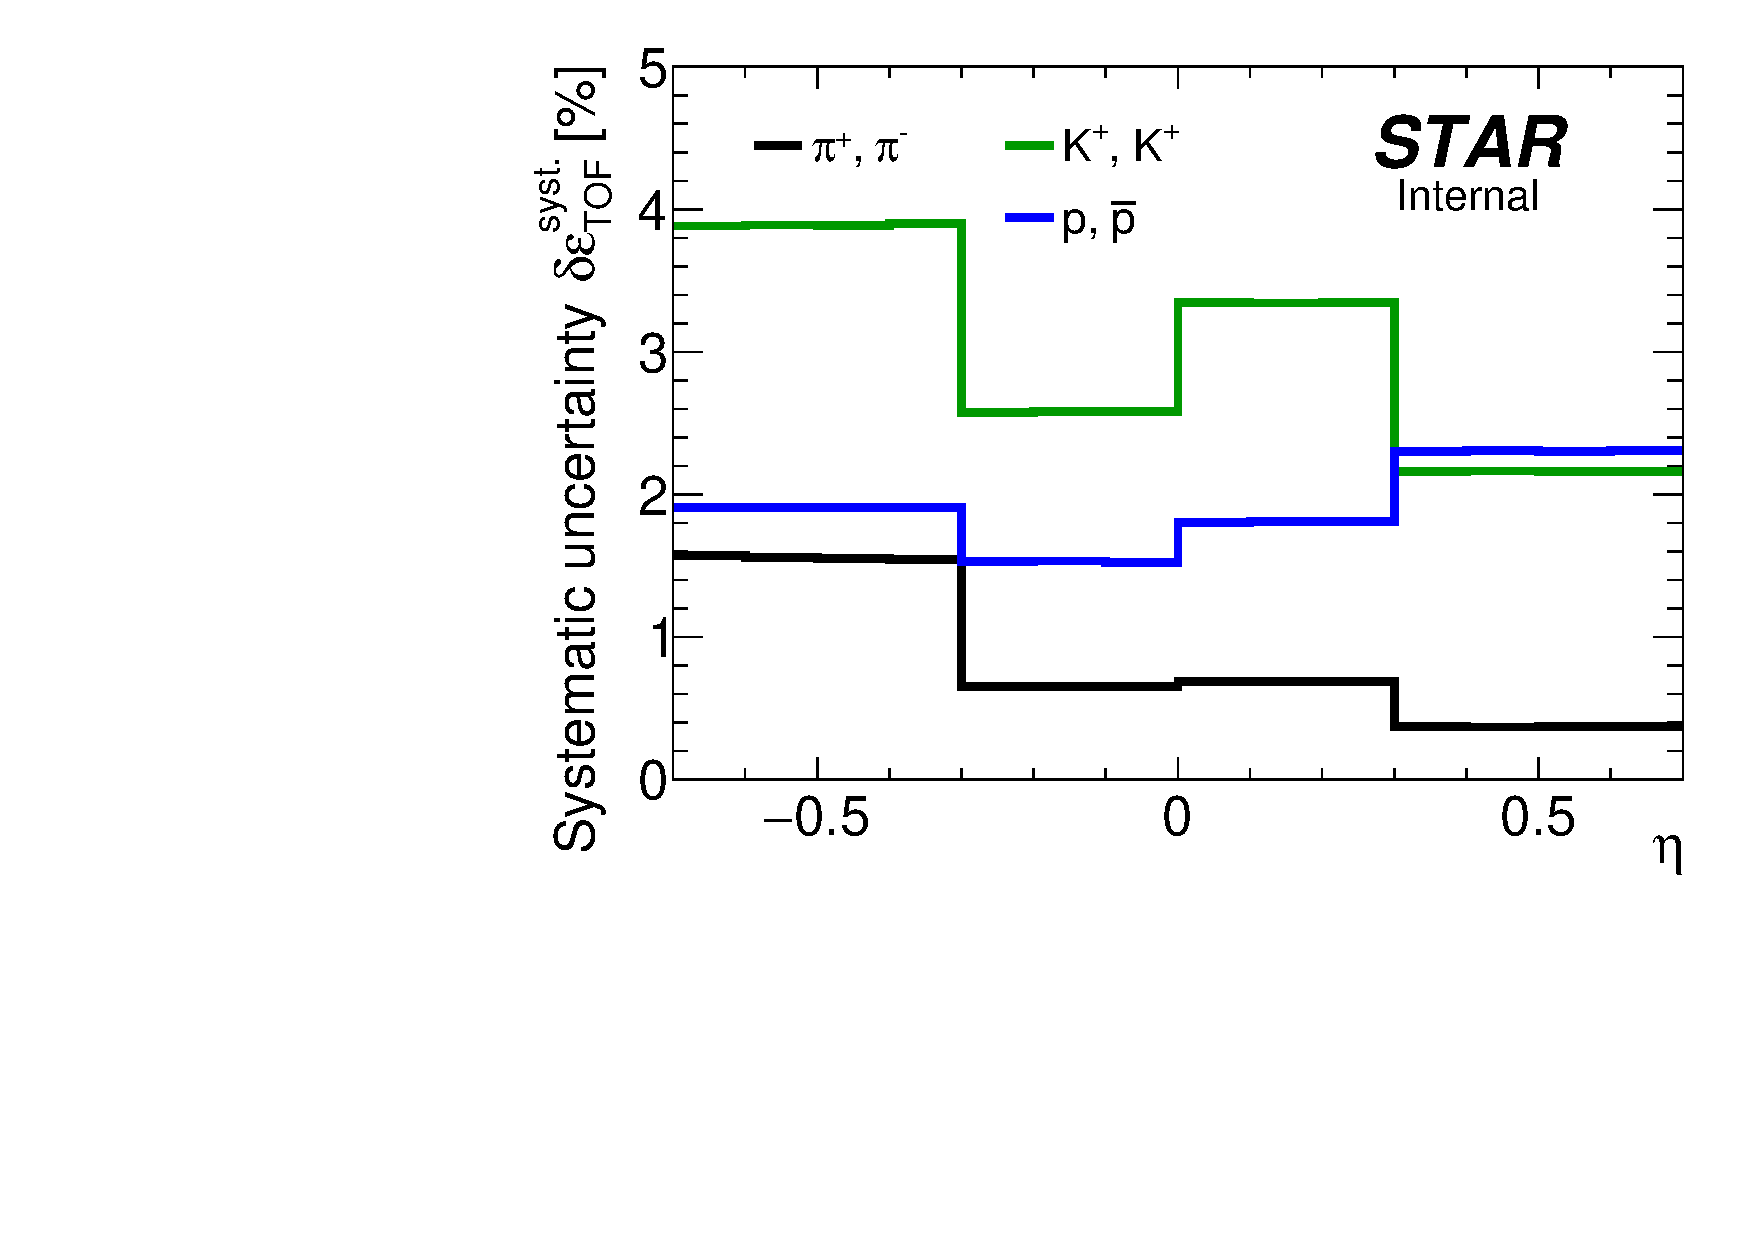
\includegraphics[width=0.49\textwidth,page=1]{chapters/chrgSTAR/img/tofEff/TofSystError_eta.pdf}
	\caption{The systematic uncertainty on TOF efficiency  related to the simulation accuracy, drawn as a function of (left) $p_\textrm{T}$ and (right) $\eta$. Figure taken from~\cite{RafalThesis}.}
	\label{fig:tofEffiSyst}
	
\end{figure}


%\FloatBarrier
\subsubsection{Embedding (Pile-Up) Effect}


The effects of pile-up on TOF efficiency is taken into account by using single particle MC embedded into Zerobias data. To estimate the systematic uncertainty of the TOF efficiency related to the~embedding procedure, the offset from the linearity of TOF efficiency  as a function of the mean BBC\_AND rate, $\langle\text{BBC\_AND}\rangle$, was used. The embedded MC was divided into two samples in which $\langle\text{BBC\_AND}\rangle$ rates differ by a factor of two: \mbox{$\langle\text{BBC\_AND}\rangle=700$~kHz} and \mbox{$\langle\text{BBC\_AND}\rangle=1400$~kHz} as shown in Fig.~\ref{fig:events_bbc_and}.
Next, it was checked whether the difference between TOF efficiency in pile-up and no-pile-up MC also changes by a factor of two between these two samples. The TOF matching efficiency is conditional and depends on TPC track reconstruction efficiency. Hence, the difference between pile-up and  no-pile-up MC was calculated as:
\begin{equation}
\Delta\epsilon_\textrm{TOF}^{1400/700\text{ kHz}}=\frac{N_\textrm{TPC-TOF}^\textrm{no-pile-up}}{N_\textrm{TPC}^\textrm{no-pile-up}}-\frac{N_\textrm{TPC-TOF}^\textrm{pile-up}}{N_\textrm{TPC}^\textrm{pile-up}}
\label{eq:tofSyst}
\end{equation}
where: $N_\textrm{TPC-TOF}^\textrm{pile-up}$ is the~umber of reconstructed tracks, matched with MC tracks and TOF hit in pile-up MC, $N_\textrm{TPC-TOF}^\textrm{no-pile-up}$ is the~number of reconstructed tracks, matched with MC tracks and TOF hit in no-pile-up MC, $N_\textrm{TPC}^\textrm{pile-up}$ is the~number of reconstructed tracks, matched with MC tracks in pile-up MC, $N_\textrm{TPC}^\textrm{no-pile-up}$ is the~number of reconstructed tracks, matched with MC tracks in no-pile-up MC.
\newline

\begin{figure}[h!]
	\centering
	\parbox{0.49\textwidth}{
		\centering
		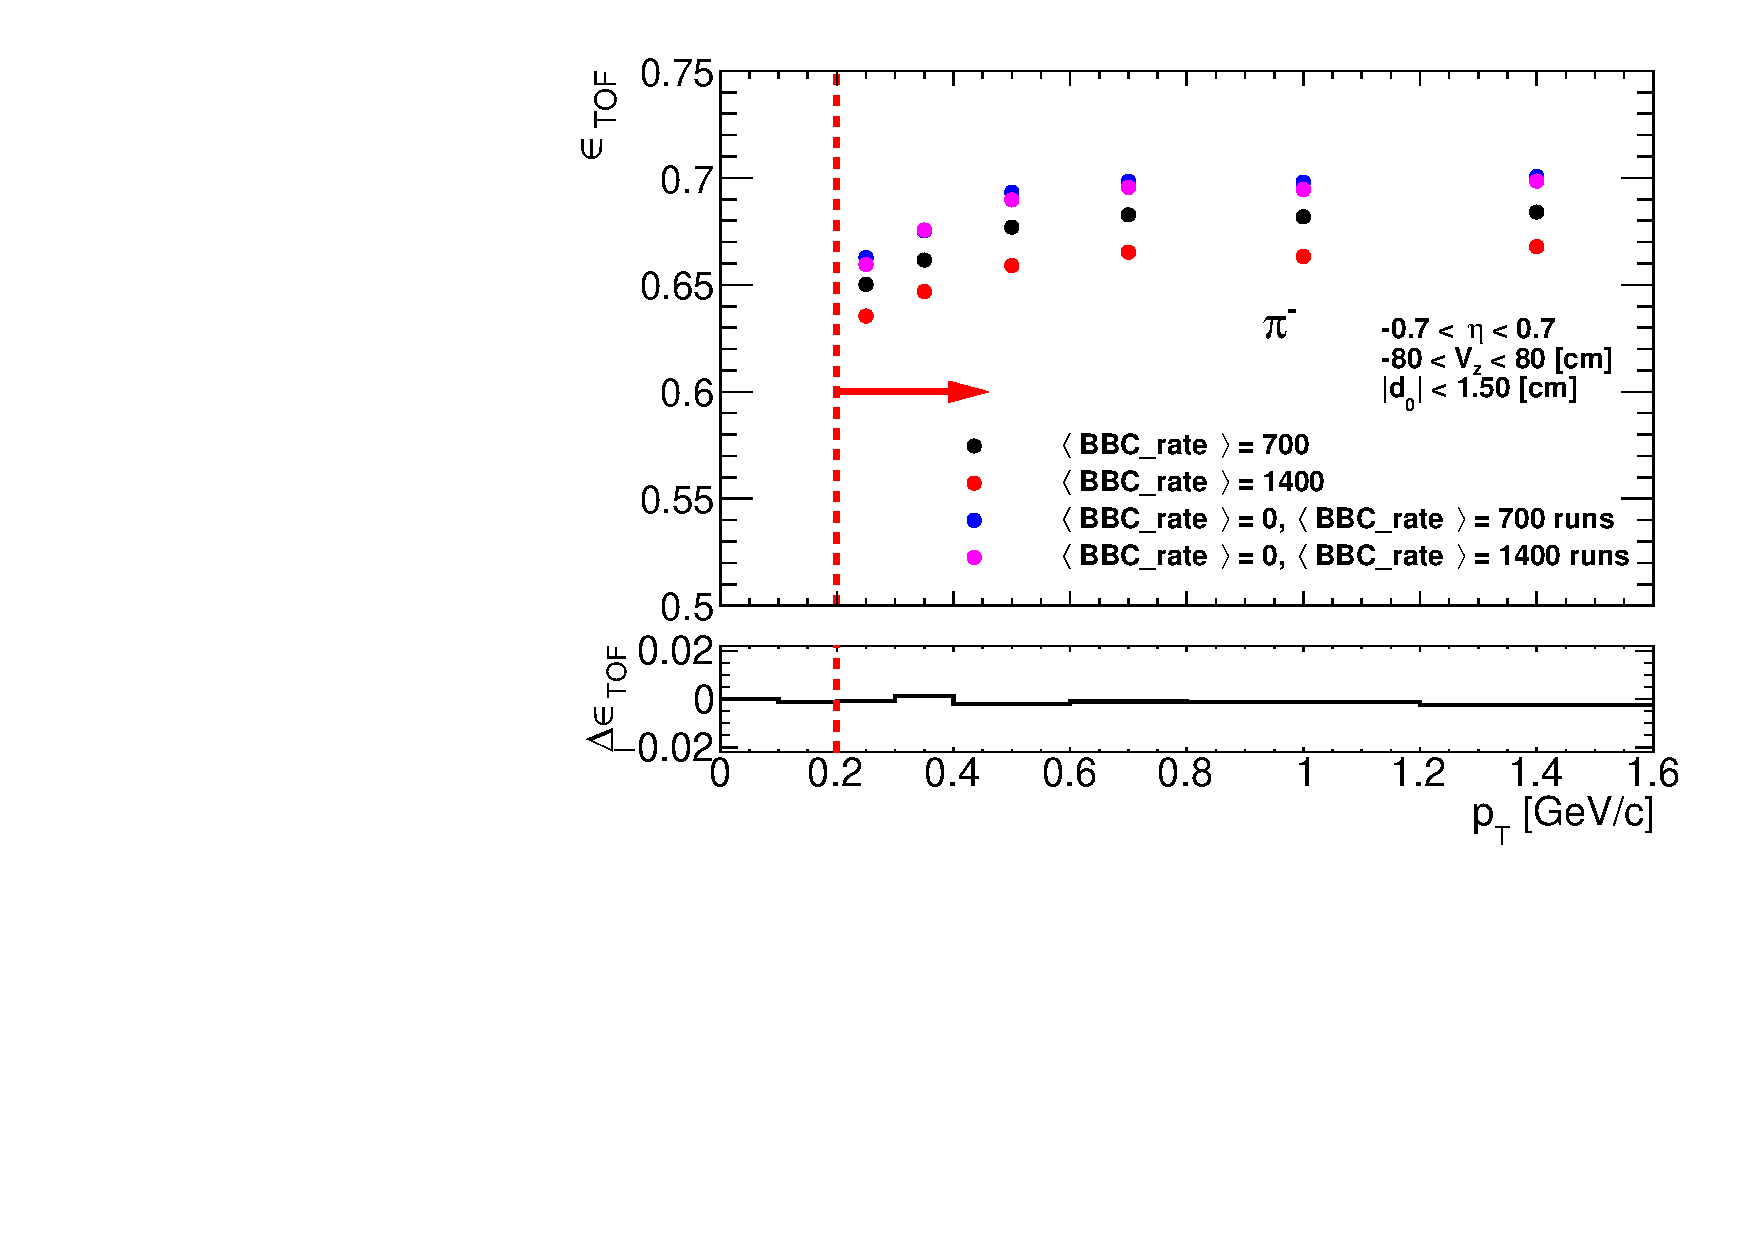
\includegraphics[width=\linewidth,page=1]{chapters/chrgSTAR/img/tofEff/tofEffi_d0_1_5_etapt_1.pdf}\\
	}~
	\parbox{0.49\textwidth}{
		\centering
		\includegraphics[width=\linewidth,page=2]{chapters/chrgSTAR/img/tofEff/tofEffi_d0_1_5_etapt_1.pdf}\\
	}%
	\caption{TOF matching efficiency for $\pi^\pm$ as a function of $p_\textrm{T}$  for embedded MC samples with \mbox{$\langle\text{BBC\_AND}\rangle=700$~kHz} and \mbox{$\langle\text{BBC\_AND}\rangle=1400$~kHz}. The efficiences from corresponding no-pile-up MC samples were also shown. Red lines and arrows indicate region accepted in the analysis.}
	\label{fig:systError1Dtof}
\end{figure}

\noindent Next the offset between high and low pile-up events was calculated with the formula:
\begin{equation}
\Delta\epsilon_\textrm{TOF} =\Delta\epsilon_\textrm{TOF}^{1400\text{ kHz}}-2\cdot\Delta\epsilon_\textrm{TOF}^{700\text{ kHz}}
\label{eq:tofSystDifference}
\end{equation}
which is shown in \cref{fig:systError1Dtof}.  The obtained value of $\Delta\epsilon_\textrm{TOF}$ is  smaller than $0.5\%$ and can be neglected in comparison with other systematic uncertainties.


%\FloatBarrier